\documentclass[11pt]{article}
\usepackage[a4paper,margin=2.3cm]{geometry}
\usepackage[T1]{fontenc}
\usepackage[utf8]{inputenc}
\usepackage{lmodern,amsmath,graphicx,xcolor,setspace,lineno}
\usepackage[round,authoryear]{natbib}
\usepackage[colorlinks=true,linkcolor=blue!50!black,citecolor=blue!50!black,urlcolor=blue!50!black]{hyperref}
\newcommand{\degr}{\ensuremath{^\circ}}
\setstretch{1.15}
\linenumbers
\pagestyle{plain}

\title{Ocean tides modulate the 26-second Gulf of Guinea microseism}
\author{Larsen Cundric\\[6pt]
\normalsize\textit{AI-generated manuscript produced using Grok Bot}\\
\normalsize\textit{Experiment initiated and guided by Larsen Cundric}}
\date{}

\begin{document}
\maketitle
\vspace{-2em}
\begin{center}\small Draft manuscript prepared in the format of \emph{Geophysical Research Letters}, 11 October 2026\end{center}

\section*{Key Points}
\begin{itemize}
\item The 26 s Gulf of Guinea microseism is tidally modulated: its power rises by about 11\% (0.47 dB) 1.6 h after M2 high water
\item The same timing is clear at stations in Cameroon, Algeria and Cape Verde and consistent at two weaker ones, so it arises at the source
\item Linear tidal water-depth effects at shelf depths are 4--40 times too weak; very shallow coupling or a nonlinear source is indicated
\end{itemize}

\section*{Plain Language Summary}
For more than sixty years seismometers around the world have recorded a faint, almost pure seismic ``hum'' with a period of about 26 seconds coming from the Gulf of Guinea, off West Africa. Its cause is still unknown. We used seven years of recordings to ask whether the hum responds to the ocean tide. It does: it is about 11\% stronger in power roughly one and a half to two hours after high tide, and weaker around low tide. The same timing is seen clearly at stations in Cameroon, Algeria and Cape Verde, and less precisely, but consistently, at stations in Uganda and on St Helena, where the hum is weak. Because stations thousands of kilometres apart agree, the effect happens where the hum is made, not near the seismometers. The rise and fall of the sea over the continental shelf is far too small to explain such a large change through the simple wave physics we tested. The source is therefore probably in very shallow water near the coast, or it responds to the tide in a strongly nonlinear way. This tidal response is a new, quantitative test for any explanation of the hum.

\begin{abstract}
\noindent A narrow 26 s seismic signal from the Gulf of Guinea has been known since the 1960s, but its source is unexplained. Using 7.4 years of data from station G.EDA (Cameroon) and six more distant stations, we show that the signal is modulated by the ocean tide. At EDA, its power varies with the principal lunar tide (M2) with an amplitude of 0.47 dB (95\% confidence interval 0.42--0.53 dB; about $\pm$11\% in power), peaking 1.6 h after high water. The modulation passes conservative null tests ($p \le 0.001$). The same lag is found at TAM (Algeria) and SACV (Cape Verde), and consistently at two weaker stations (combined 1.8 h; 1.5--2.1 h), so it arises at the source. The amplitude grows with tidal range, consistent with proportional scaling. Linear effects of tidal water depth at shelf depths are 4--40 times too weak, pointing to very shallow coupling or a nonlinear source.
\end{abstract}

\section{Introduction}
Seismometers worldwide record a narrow spectral peak near 26 s period (0.038 Hz) that comes from the Gulf of Guinea. Long-period microseisms of 26--27 s were first reported as a worldwide ``storm'' by \citet{oliver1962}. \citet{holcomb1980,holcomb1998} showed that a 26 s spectral line is a recurring feature of the background, and \citet{shapiro2006} located its source in the Bight of Bonny. \citet{xia2013} found two separate persistent sources, near 0.038 and 0.036 Hz, and related signals include a 16 s persistent tremor \citep{xia2020,takano2025} and gliding tremors \citep{bruland2023}.

What generates the signal is still debated. One view is that long-period ocean swell couples to the seafloor in shallow water \citep{bernard1990}, the standard mechanism for primary microseisms \citep{hasselmann1963,ardhuin2018} (the more common secondary microseisms occur at half the wave period; \citealp{longuethiggins1950}). Others argue for a solid-Earth source: a crack network driven by random processes \citep{chen2022}, or vibrating thin crustal plates above magma sills \citep{xia2024}. Most recently, \citet{poli2026} showed that bursts of 26 s energy follow the arrival of long-period swell from Southern Ocean storms, and modelled the source as resonating fluid-filled cracks triggered by swell.

The response to ocean tides is a classical way to probe how a seismic source reacts to small, known forcing \citep[e.g.,][]{rubinstein2008}, but it has not, to our knowledge, been tested for the 26 s signal. Replying to reviewers, \citet{poli2026} argued that tidal depth changes of a few metres should not affect very long swell in tens of metres of water, while noting that tides could modulate the surf zone. \textbf{Here we show that the 26 s signal is modulated by the tide: its power is about 11\% higher roughly 1.6--1.8 h after high water, at the source, and the change scales with tidal range.} We then show that simple linear wave physics at shelf depths cannot produce an effect this large.

\section{Data and Methods}
\subsection{Seismic data and the line-minus-background metric}
We use vertical long-period records (channel LHZ, 1 sample/s) from G.EDA (Cameroon; 240 km from a nominal source point at 4\degr N, 8\degr E) for 2019-05-04 to 2026-09-28, and G.TAM (Algeria; 2096 km) for 2022-03 to 2026-09. For a common period, 2022-03 to 2024-02, we add II.MBAR (Uganda; 2580 km), II.SHEL (St Helena; 2677 km), II.ASCN (Ascension; 2812 km), GE.WIN (Namibia; 3101 km) and II.SACV (Cape Verde; 3670 km) (Figure~\ref{fig:map}). Instrument responses were removed with ObsPy \citep{beyreuther2010}.

We computed spectra in 3-h windows advanced in 1-h steps. Windows with earthquakes or glitches were rejected (20--30 mHz power above five times its 15-day running median, or an extreme peak-to-median amplitude ratio); at EDA 38,888 of 52,547 windows (74.0\%) remain. We call the line ``detected'' in a window when its signal-to-noise ratio (SNR) exceeds the value reached in only 1\% of windows in a nearby line-free band (30--32.5 mHz). Power is expressed in decibels (dB; ten times the base-10 logarithm of a power ratio). An M2 amplitude of 0.47 dB therefore means that power swings between about 11\% above and 10\% below its mean.

Our main metric does not depend on detection and is computed for every retained hour. We take the power in a fixed band on the line (37.5--38.6 mHz, in dB) and subtract the part that can be predicted, by linear regression, from the power in two neighbouring background bands (20--24 s and 29--34 s periods). This ``line-minus-background'' (LMB) power removes noise that the line shares with its spectral surroundings, such as local weather, site and ocean noise (EDA regression coefficients 0.24 and 0.49). The 29--34 s band at the two strongest stations is itself weakly modulated near the line's tidal phase (full span: 0.21 dB at $+0.2$ h at EDA, 0.17 dB at $+1.1$ h at TAM), so LMB amplitudes are conservative; raw line power gives 0.548 dB at EDA and 0.473 dB at TAM.

\subsection{Tides}
The tide reference is the University of Hawaii Sea Level Center (UHSLC) research-quality hourly record at Port Sonara (Limbe, Cameroon; 4.01\degr N, 9.13\degr E) for 2008-06 to 2011-06 \citep{uhslc}. A harmonic fit with UTide \citep{codiga2011,pawlowicz2002} explains 98.9\% of the variance, with an amplitude of 0.59 m for M2, the principal lunar semidiurnal tide (period 12.42 h), and 0.21 m for S2, the principal solar semidiurnal tide. We used this fit to predict the tide for 2019--2026; no gauge record from that period is available. Fits at S\~ao Tom\'e and Lagos place M2 high water within $-0.18$ and $+0.29$ h of Port Sonara. All lags below are hours after predicted M2 high water at Port Sonara.

\subsection{Statistics}
Each hourly series was high-pass filtered (by subtracting a 72-h running median) and fitted by least squares with sinusoids at the main tidal frequencies (M2, S2, N2, K1, O1, Q1, M4, S1 and S3). For each constituent this gives an amplitude (in dB, half the peak-to-trough range) and a lag (time of maximum). Confidence intervals come from a moving-block bootstrap with 30-day blocks \citep{kunsch1989}; 15-day blocks give the same results. We tested significance against phase-randomised surrogate series \citep{theiler1992} and, most conservatively, against ``block-resampled'' surrogates, in which 15- or 30-day blocks of data are moved to random times relative to the tide (1000 realisations each). Multi-station lags were combined by inverse-variance weighting, with a bootstrap that resamples the same blocks at all stations to preserve correlations between them.

Tidal range varies over the fortnightly spring--neap cycle, from large spring tides to small neap tides. To test whether the response follows this cycle we (i) measured the response separately in five bins of tidal range (the semidiurnal envelope $E$), and (ii) fitted a model in which the M2-band response grows linearly with relative range $e=E/\bar E-1$. Its scaling index $\gamma$ is 0 for a constant response and 1 for a response proportional to tidal range. The ratio of the S2 to M2 responses, compared with the same ratio in the tide, gives an independent version of the test.

\subsection{Toy model}
To estimate the size of linear water-depth effects we computed the M2 modulation of several quantities for 26 s swell under a 0.59 m M2 tide: bottom pressure and bed orbital velocity (linear waves with shoaling), primary-microseism forcing over a wavy bottom with spectrum $F_B\propto k^{-2}$ or $k^{-3}$ \citep{hasselmann1963,ardhuin2018}, depth-limited (breaking) forcing, and wave--current interaction for a standing tide.

\section{Results}
\subsection{A tidal signal in the 26 s line}
The line is detected in 31.0\% of retained hours at EDA (median period 26.341 s, 95\% CI 26.336--26.347 s; Figure~\ref{fig:map}c) and in 14.1\% at TAM. In the LMB periodogram the M2 frequency stands out at both stations, with peak-to-median power ratios of 147 (EDA) and 130 (TAM), against 95\% surrogate band maxima of 8.7 and 6.6 (Figure~\ref{fig:tide}a,b). At EDA the M2 amplitude is 0.473 dB (95\% CI 0.422--0.529 dB) with a lag of $+1.63$ h (1.46--1.82 h). None of the 1000 block-resampled surrogates reaches this amplitude for either block length ($p\le0.001$; $z=17.3$ and 13.5 for 15- and 30-day blocks), and neither do any of 500 phase-randomised surrogates. Allowing for autocorrelation, the 38,888 hours are worth about 17,336 independent samples. TAM gives 0.398 dB (0.346--0.455 dB) at $+1.66$ h (1.45--1.89 h). Binned by tidal phase, power follows a smooth, nearly sinusoidal cycle at EDA, TAM and SACV (Figure~\ref{fig:tide}c).

The result does not depend on the metric. Raw line power (0.548 dB, $+1.3$ h), SNR (0.391 dB, $+1.7$ h) and the detection rate all show it; detection rises from about 26\% near low water to 36\% near high water (M2 amplitude 5.5 percentage points). The S2 (0.168 dB, $+2.2$ h) and N2 (0.075 dB, $+2.4$ h) terms are also significant, while M4 is small (0.033 dB). Leaving out any one calendar year changes the EDA amplitude only to 0.448--0.492 dB and the lag to 1.57--1.67 h. Single years range from 0.284 to 0.602 dB, lowest in 2024--2026, with lags of 1.33--1.85 h. Adding ERA5 wave height and peak period \citep{hersbach2020} as covariates leaves the M2 term unchanged (0.473 dB).

\subsection{The same timing at distant stations: a source effect}
In the common period 2022-03 to 2024-02 the M2 term passes all three null tests at EDA, TAM and SACV, and also, more weakly, at SHEL and MBAR (Figure~\ref{fig:phasors}). The lags are $+1.75$ h (95\% CI 1.31--2.14 h) at EDA, $+1.75$ h (1.47--2.10 h) at TAM and $+1.82$ h (1.25--2.41 h) at SACV, with amplitudes of 0.513, 0.445 and 0.274 dB. SHEL ($+1.99$ h, 0.96--2.82 h; 0.159 dB) detects the line in only 3.4\% of hours. MBAR ($+2.40$ h, 1.00--3.57 h; 0.109 dB) is marginal ($p\approx0.03$). The five lags agree statistically ($p=0.88$), with a weighted mean of $+1.80$ h (1.49--2.10 h), dominated by TAM, EDA and SACV. These stations lie 240--3670 km from the source at azimuths from 96\degr\ to 353\degr, with different local tides, oceanic settings and noise. Their background noise does not share the line's timing: the 20--24 s bands peak 6.0--8.0 h after high water at all seven stations, and the 29--34 s bands peak 6--10 h after high water at MBAR, SHEL, ASCN and SACV. A common timing of the line at such distances, but not of the background, places the modulation at the source rather than near the receivers or along the paths. II.ASCN and GE.WIN detect the line in only about 2\% and 3\% of hours and show no significant M2 term ($p\approx0.3$--0.4). They are uninformative rather than contradictory.

\subsection{Scaling with tidal range}
The response is larger at spring tides than at neap tides (Figure~\ref{fig:sn}a). Across five bins of tidal range (mean envelope 0.34--0.84 m), the EDA response rises from 0.35 to 0.66 dB. A constant response is rejected ($p=4\times10^{-4}$; TAM $p=7\times10^{-4}$), while proportional scaling is acceptable ($p=0.32$; TAM 0.28). The scaling index is $\gamma=0.70$ (0.41--0.99) at EDA and 0.68 (0.35--1.05) at TAM over the full records, and 0.96 (0.56--1.37) at EDA when only the spring--neap (M2+S2) part of the range variation is used. The S2/M2 response ratio at EDA (0.355) matches that of the tide (0.360), an admittance of 0.99 (0.70--1.30). In short, $\gamma\approx0.7$--1, and proportional scaling is not excluded.

We do not regard values below 1 as robust. They depend on the metric (raw line power gives $\gamma=1.01$ at EDA but 0.32 at TAM), and they come mostly from the weaker monthly (lunar perigee, N2) part of the range variation. Plausible errors in the predicted tide bias $\gamma$ by only about 6--12\% (Supporting Information). A purely lunar test is weak, because the lunar-only envelope varies by only about $\pm$20\%. With a complete lunar envelope it gives $\gamma=0.88$ (0.07--1.72) at TAM, consistent with proportionality, and 0.45 ($-0.20$ to 1.16) at EDA, which is inconclusive. In 2-yr windows $\gamma$ is poorly constrained (standard deviation 0.27--0.32 at EDA and TAM, 0.44--0.50 at SACV). The 2022--2024 values are low at all three stations (SACV $-0.26$, $-0.88$ to 0.52), partly because the stations share noise. We cannot distinguish this from a modest real change in the source's tidal sensitivity.

\subsection{Spectral structure}
The nearby 28 s line is also modulated, more weakly and slightly later (0.16 dB at $+2.5$ h at EDA, 0.17 dB at $+2.3$ h at TAM, after removing local background). Both components of the 26 s doublet are modulated by the same amount (EDA 0.61 and 0.63 dB in raw power). We find no robust tidal change in the line's frequency. An apparent M2 frequency term (14 $\mu$Hz at EDA, 38 $\mu$Hz at TAM) peaks near the time of lowest SNR and is larger at the lower-SNR station. It is not significant for high-SNR detections at EDA ($p=0.17$) or at EDA in 2022--2026 ($p=0.5$). We attribute it to an SNR-dependent bias of the frequency estimate, but cannot exclude a real modulation of $\sim$10--15 $\mu$Hz (Supporting Information).

\section{Discussion}
\subsection{Too large for linear depth effects}
At EDA the tide changes the line's power by about $\pm$11\%. Linear effects of a 0.59 m M2 tide on 26 s swell are much smaller at shelf depths (Figure~\ref{fig:sn}b). Primary-microseism forcing over a wavy bottom changes by only 0.011--0.112 dB at 20--50 m depth, 4--40 times less than observed. Bottom pressure and bed orbital velocity change with the wrong sign (larger at low water). Wave--current interaction gives at most 0.07 dB at 20--50 m and peaks 3.1 h after high water. These linear mechanisms reach $\sim$0.45 dB only in water $\sim$3--8 m deep. Depth-limited (breaking) forcing reaches 0.51 dB at 10 m mean depth, but applies only in the surf zone. This agrees with the expectation of \citet{poli2026} that metre-scale depth changes should not affect swell in tens of metres of water. The tidal signal must therefore arise where the water is very shallow (surf zone, estuaries, tidal flats) or through a strongly nonlinear source. For example, a source whose output grows exponentially with bottom pressure, $\propto\exp(\Delta p/p_0)$, needs $p_0\approx47$--64 kPa to give the observed 0.40--0.55 dB from a tidal pressure amplitude of 5.9 kPa.

\subsection{What kind of nonlinearity?}
Harmonics limit the form of any nonlinear response. The observed ratio of the quarter-diurnal M4 term to M2 at EDA (0.071) is close to that of the tide itself (0.054). A response that switches on above a threshold, or is clipped on one side, would give M4/M2 of 0.14--0.32 and is excluded. A gently saturating, symmetric response (e.g.\ $\tanh(h/0.6\,\mathrm{m})$ of tidal height $h$) gives $\gamma=0.70$ with M4/M2 of 0.046 and is allowed. A response that is linear in power but measured in dB, or one driven by tidal current rather than height, gives $\gamma\ge1$. However, as noted above, $\gamma<1$ is not itself robust.

\subsection{The lag}
Maximum power 1.6--1.8 h after M2 high water is not explained by tidal height alone. The tide is nearly in phase across the gauges we examined (within $\pm$0.3 h), so the lag must come from the source physics or from a local delay. A height-driven term plus an opposing-current term (which peaks at $+3.1$ h for a standing tide) reproduces it if their amplitudes are in the ratio 1.16--1.60. Alternatives are delayed tides in estuaries and creeks, which lag the open coast, or a delayed (e.g.\ poroelastic) response. We cannot test these without regional tidal-current data.

\subsection{Implications and tests}
Any explanation of the 26 s signal must now account for a source-side modulation of about $\pm$11\% in power that roughly scales with tidal range and lags high water by 1.6--1.8 h, alongside the swell control shown by \citet{poli2026}. Swell interacting with very shallow coastal topography would naturally produce both, but a nonlinear, swell-triggered resonator remains possible. Decisive tests would use (i) the timing relative to tidal currents from a validated regional tide model, (ii) the tidal modulation of swell-driven bursts as a function of swell height, and (iii) coastal or ocean-bottom pressure records near the proposed source. As a side remark, both components of the 26 s doublet---whose splitting was already suggested by \citet{holcomb1998}---share the same tidal modulation. The dominant component switched from $\sim$26.3 s to $\sim$26.5 s in 2025 (Supporting Information).

\subsection{Limitations}
The tide reference is a harmonic prediction from one gauge record (2008--2011), not contemporaneous observations. Modulation at distant stations is small (0.1--0.3 dB); MBAR is marginal and SHEL rarely detects the line. Station noise is correlated (hourly LMB correlation $\sim$0.5), so stations are not fully independent. The near-line background is itself weakly modulated at EDA and TAM, and $\gamma$ depends on how background is removed. The toy model is linear and deliberately simple.

\section{Conclusions}
The 26 s Gulf of Guinea microseism is modulated by the ocean tide. At the near-source station EDA its power varies by 0.47 dB (about $\pm$11\%), peaking 1.6 h after M2 high water. The result survives conservative null tests, leave-one-year-out tests and changes of metric. The same timing is found clearly at TAM and SACV, up to 3670 km away, and consistently at SHEL and MBAR, so the modulation is a property of the source. Its amplitude grows with tidal range ($\gamma\approx0.7$--1; proportional scaling not excluded). Linear depth effects at shelf depths are 4--40 times too small, pointing to coupling in very shallow water or to a nonlinear, mildly saturating source; threshold-like clipping is excluded by the weak M4 response.

\section*{Open Research}
Seismic data were obtained through FDSN web services: network G (GEOSCOPE; \citealp{geoscope}; stations EDA and TAM, location 00, channel LHZ) from RESIF (\url{https://ws.resif.fr}); network II (\citealp{gsnII}; MBAR, SHEL, ASCN and SACV, location 00, LHZ) from EarthScope (\url{https://service.earthscope.org}); and network GE (GEOFON; \citealp{geofon}; WIN, LHZ) from GEOFON (\url{https://geofon.gfz.de}). Hourly research-quality sea level for Port Sonara (UHSLC station 816), S\~ao Tom\'e (225), Lagos (233) and Praia (222) is from the University of Hawaii Sea Level Center \citep{uhslc}. ERA5 wave parameters \citep{hersbach2020} at 3\degr N, 8\degr E and 15\degr N, 23.5\degr W were obtained through the Open-Meteo API \citep{zippenfenig2024}. Coastlines are from Natural Earth \citep{naturalearth}. Processing used ObsPy \citep{beyreuther2010}, the Python port of UTide \citep{utidepy,codiga2011}, NumPy \citep{harris2020}, SciPy \citep{virtanen2020} and Matplotlib \citep{hunter2007}. The analysis scripts and derived hourly series are available from the author on request.

\section*{AI-Use Disclosure}
This manuscript was generated with Grok Bot, an AI agent, in an experiment initiated and guided by Larsen Cundric. The AI system: (i) located and downloaded the seismic waveforms, station metadata, tide-gauge records, wave-reanalysis series and coastline data through public web services; (ii) wrote all analysis code, including spectral estimation, detection and quality control, tidal fitting and prediction, and harmonic regression; (iii) designed and ran the statistical tests (block bootstrap, phase-randomised and block-resampled nulls, spring--neap, sideband and robustness diagnostics); (iv) formulated and computed the toy model of tidal depth effects; (v) searched the literature, read the available papers and checked the bibliographic details of every reference against Crossref, DataCite or publisher records; (vi) produced all figures; and (vii) drafted and revised the text, including this disclosure. Larsen Cundric chose the topic, set the scope and working constraints, steered the priorities and requested revisions. The author initiated and guided this experiment but has not independently verified the analysis; the paper has not been reviewed by a domain expert.

\bibliographystyle{plainnat}
\bibliography{refs}

\clearpage
\begin{figure}[p]
\centering
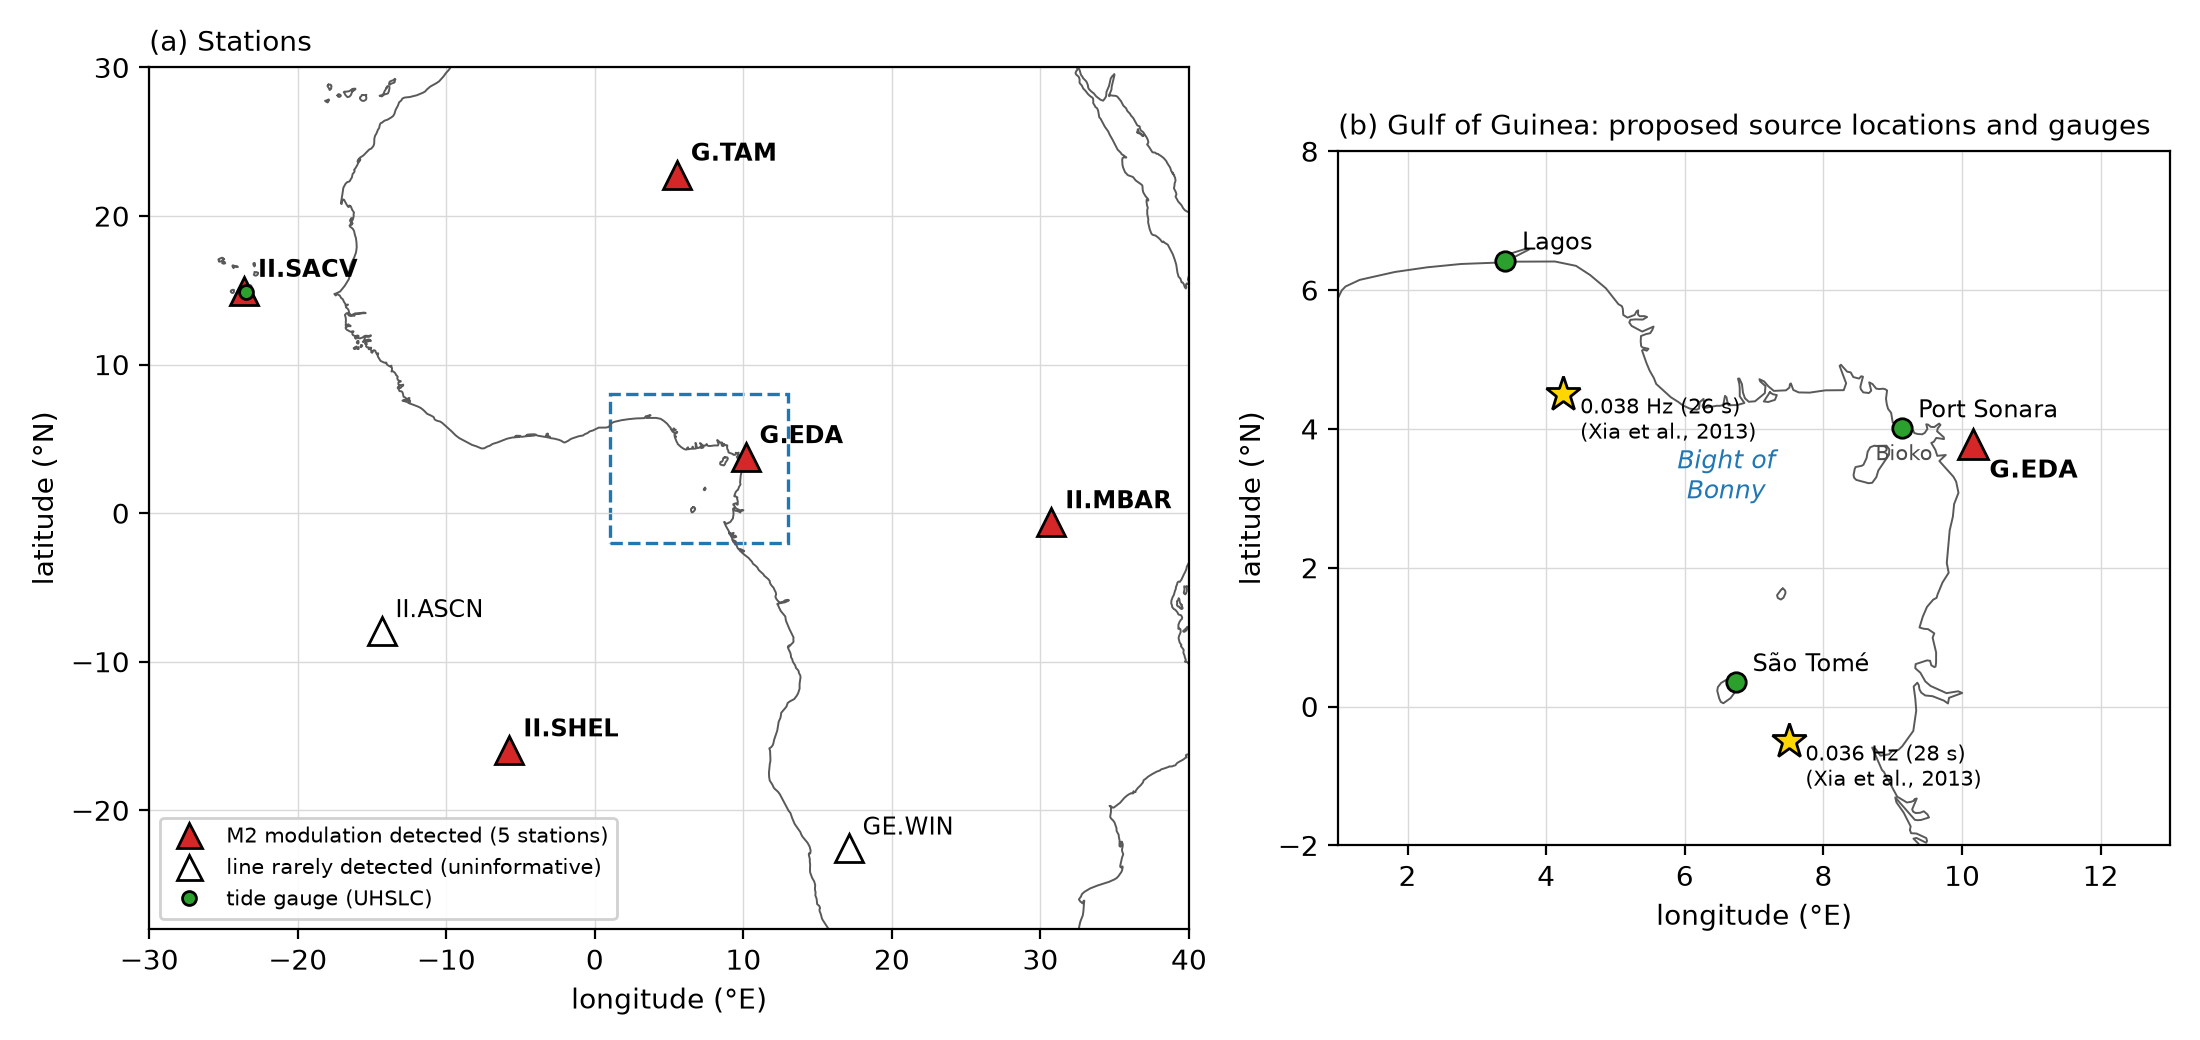
\includegraphics[width=\textwidth]{figs/fig1a_map.png}\\[2pt]
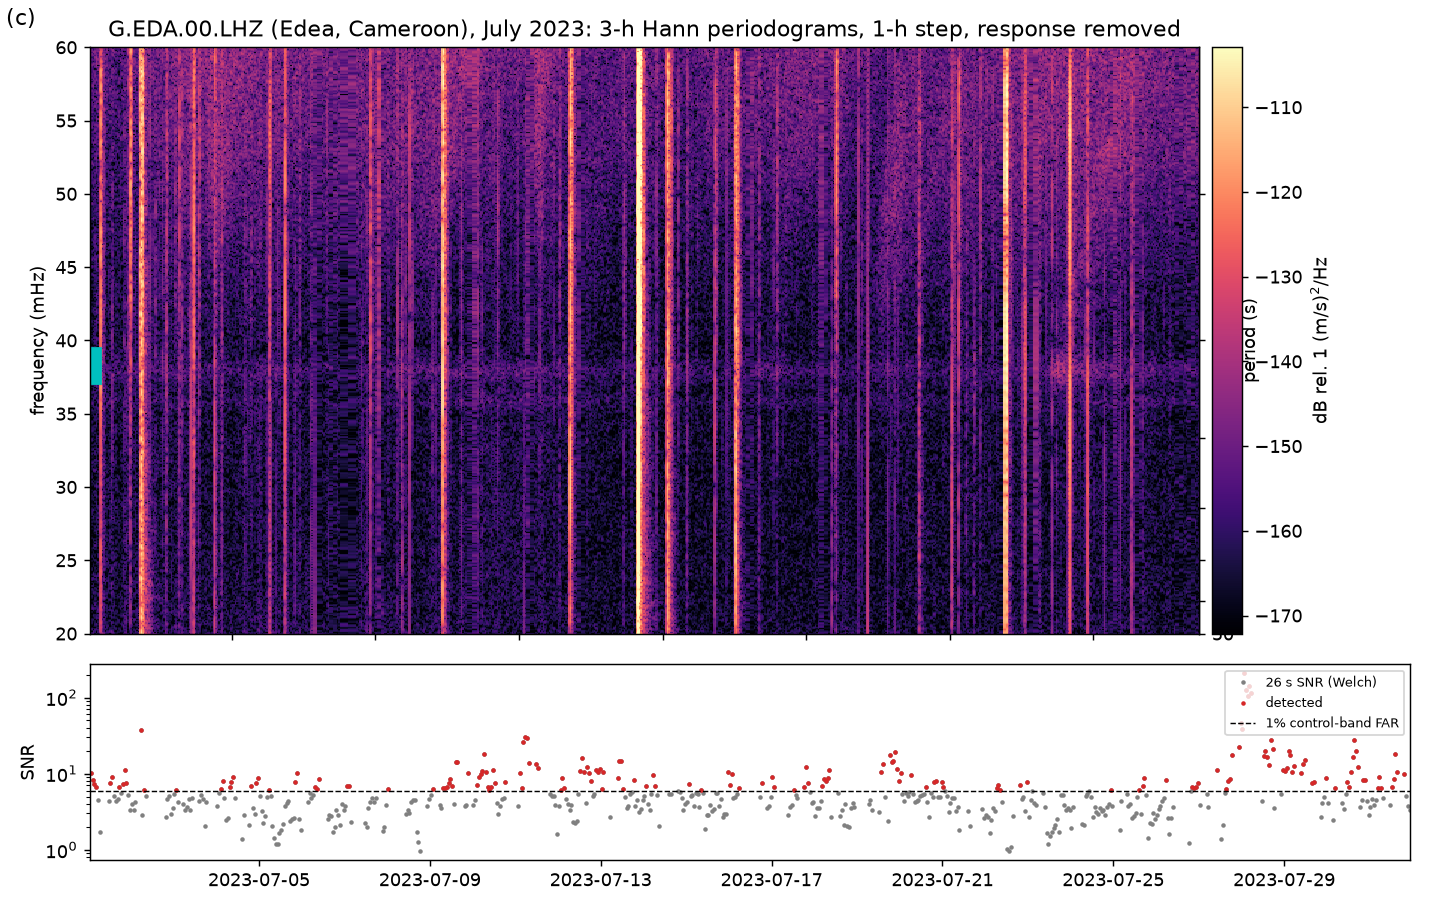
\includegraphics[width=0.92\textwidth]{figs/fig1b_spectrogram.png}
\caption{(a) Stations used. Red triangles: stations where the M2 modulation is detected; open triangles: stations where the 26 s line is rarely detected; green circles: UHSLC tide gauges. (b) The Gulf of Guinea, with the Port Sonara (Limbe), S\~ao Tom\'e and Lagos gauges and the 0.038 Hz and 0.036 Hz source locations of \citet{xia2013}. (c) Spectrogram at G.EDA for July 2023 (3-h windows, 1-h step), showing the 26 s line near 38 mHz, and the line's SNR with detections above the 1\% false-alarm level (dashed).}
\label{fig:map}
\end{figure}

\begin{figure}[p]
\centering
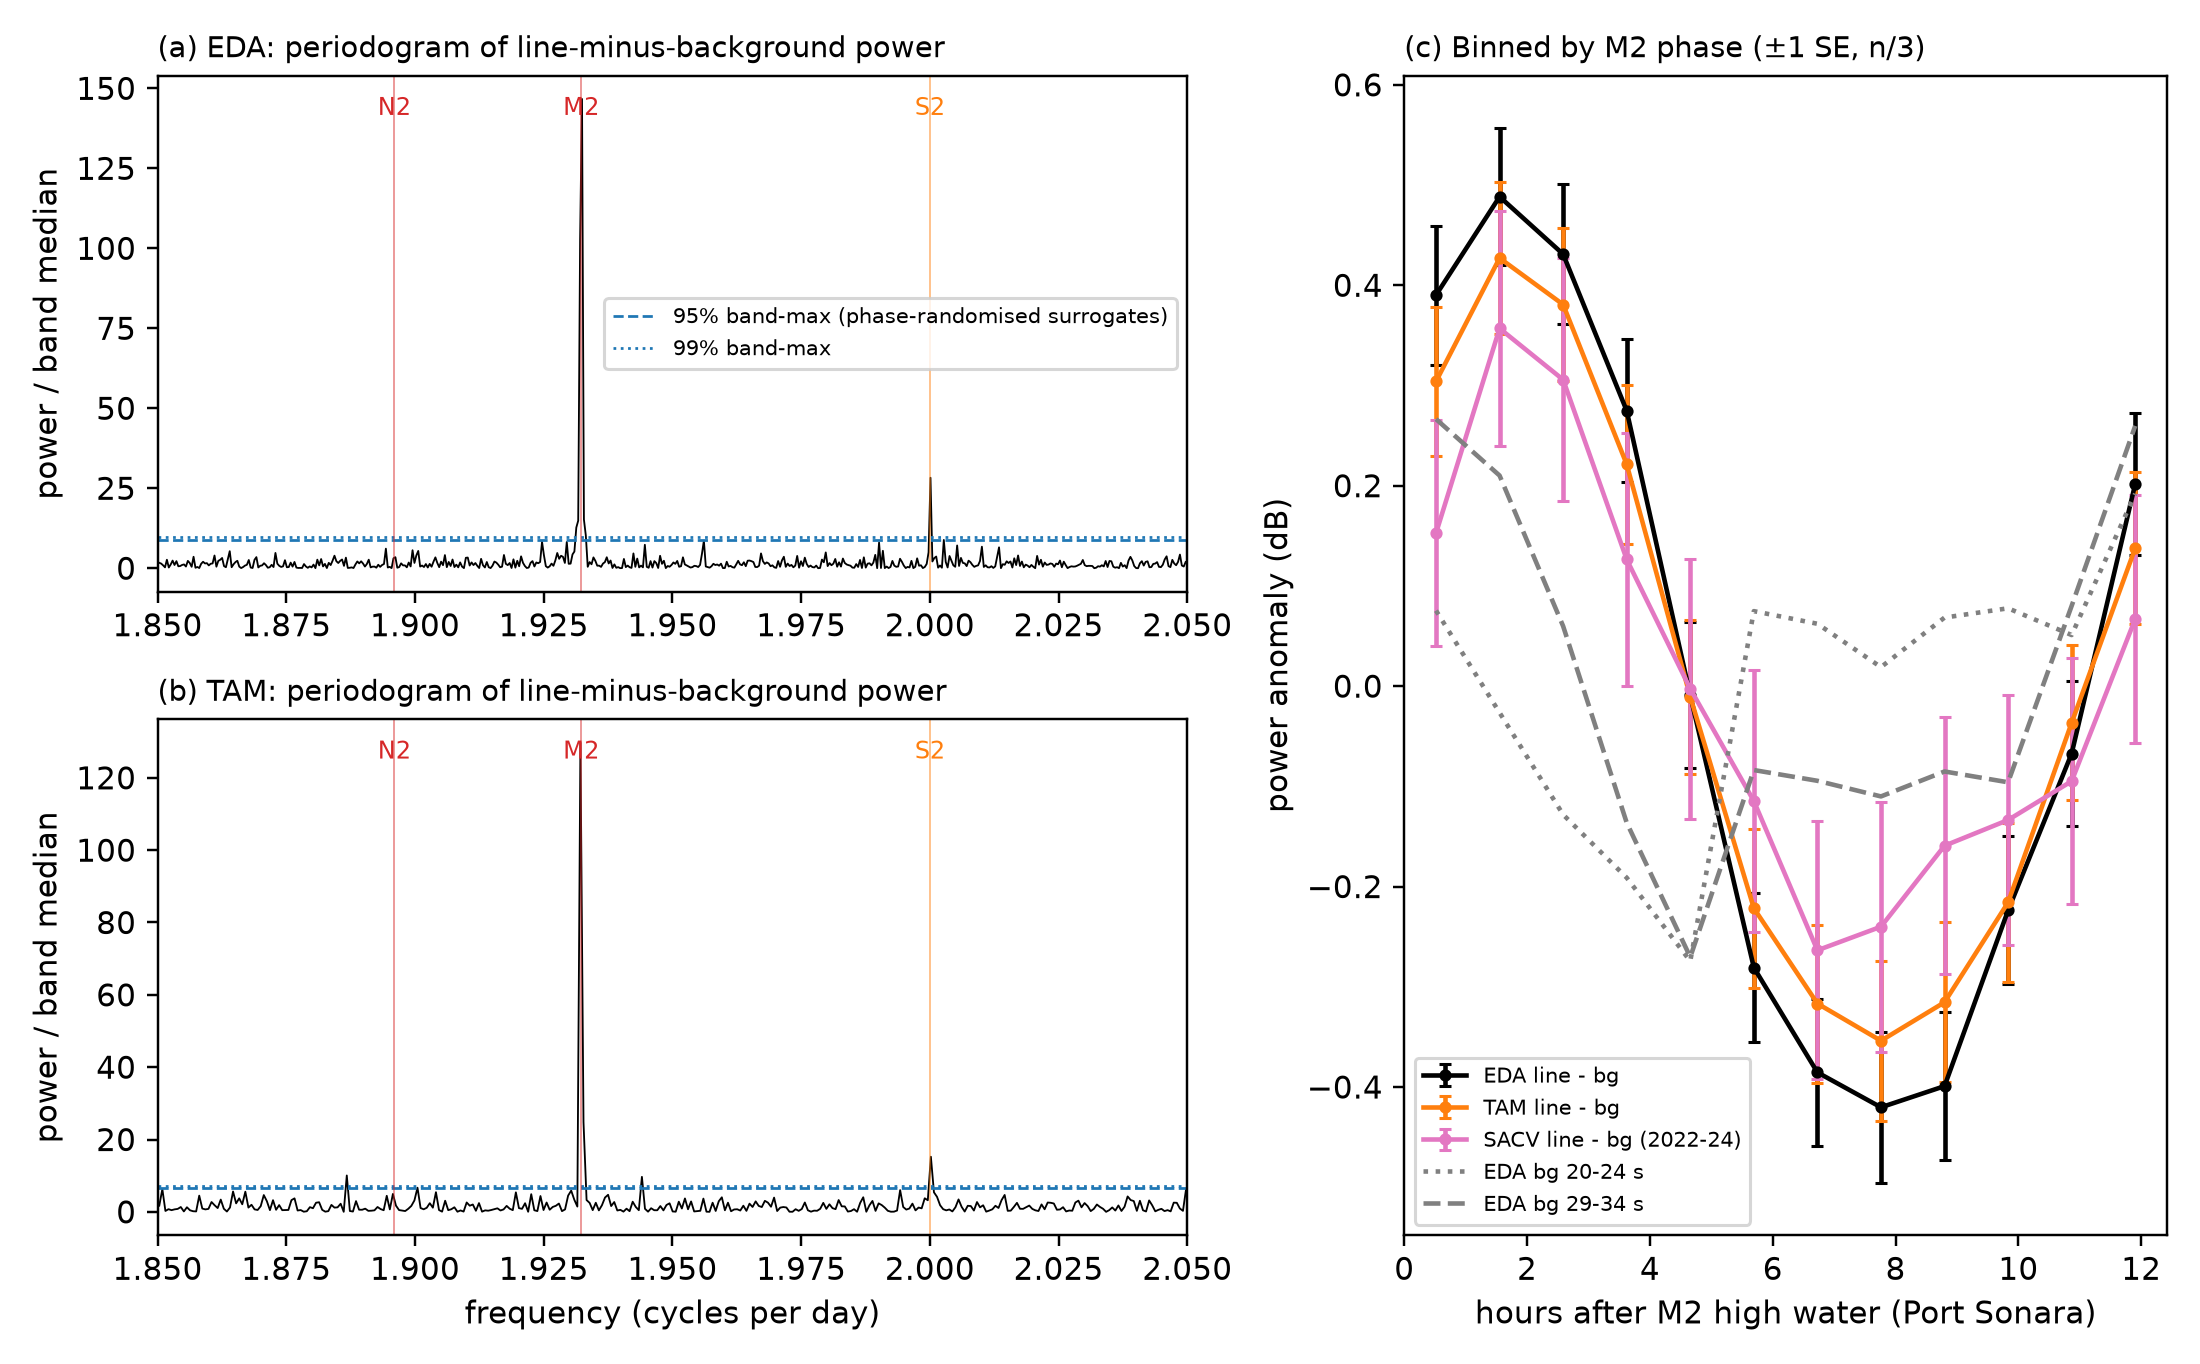
\includegraphics[width=\textwidth]{figs/fig2_tidal_periodogram_phase.png}
\caption{Tidal modulation of line-minus-background (LMB) power. (a, b) Periodograms of the hourly LMB series at EDA (2019--2026) and TAM (2022--2026) around the semidiurnal tidal band, normalised by the band median. Horizontal lines are the 95\% and 99\% band maxima of 200 phase-randomised surrogates. (c) LMB power binned by M2 tidal phase (hours after M2 high water at Port Sonara; 12 bins, $\pm1$ standard error, with sample size divided by 3 for autocorrelation) at EDA, TAM and SACV (2022--2024), and the two EDA background bands.}
\label{fig:tide}
\end{figure}

\begin{figure}[p]
\centering
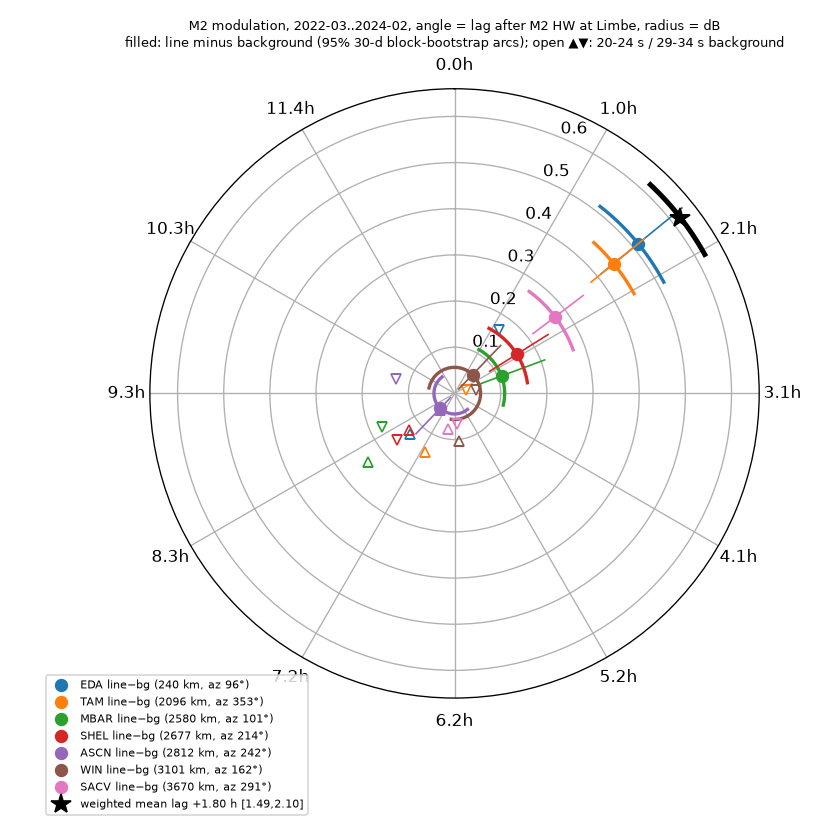
\includegraphics[width=0.78\textwidth]{figs/fig3_multistation_phasors.png}
\caption{M2 modulation of LMB power at all seven stations over the common period 2022-03 to 2024-02. Angle: lag after M2 high water at Port Sonara; radius: amplitude (dB). Filled circles with arcs: LMB with 95\% 30-day block-bootstrap intervals in amplitude and lag. Open triangles: the 20--24 s and 29--34 s background bands of each station. Star: weighted mean lag of the five stations with significant modulation, $+1.80$ h (1.49--2.10 h).}
\label{fig:phasors}
\end{figure}

\begin{figure}[p]
\centering
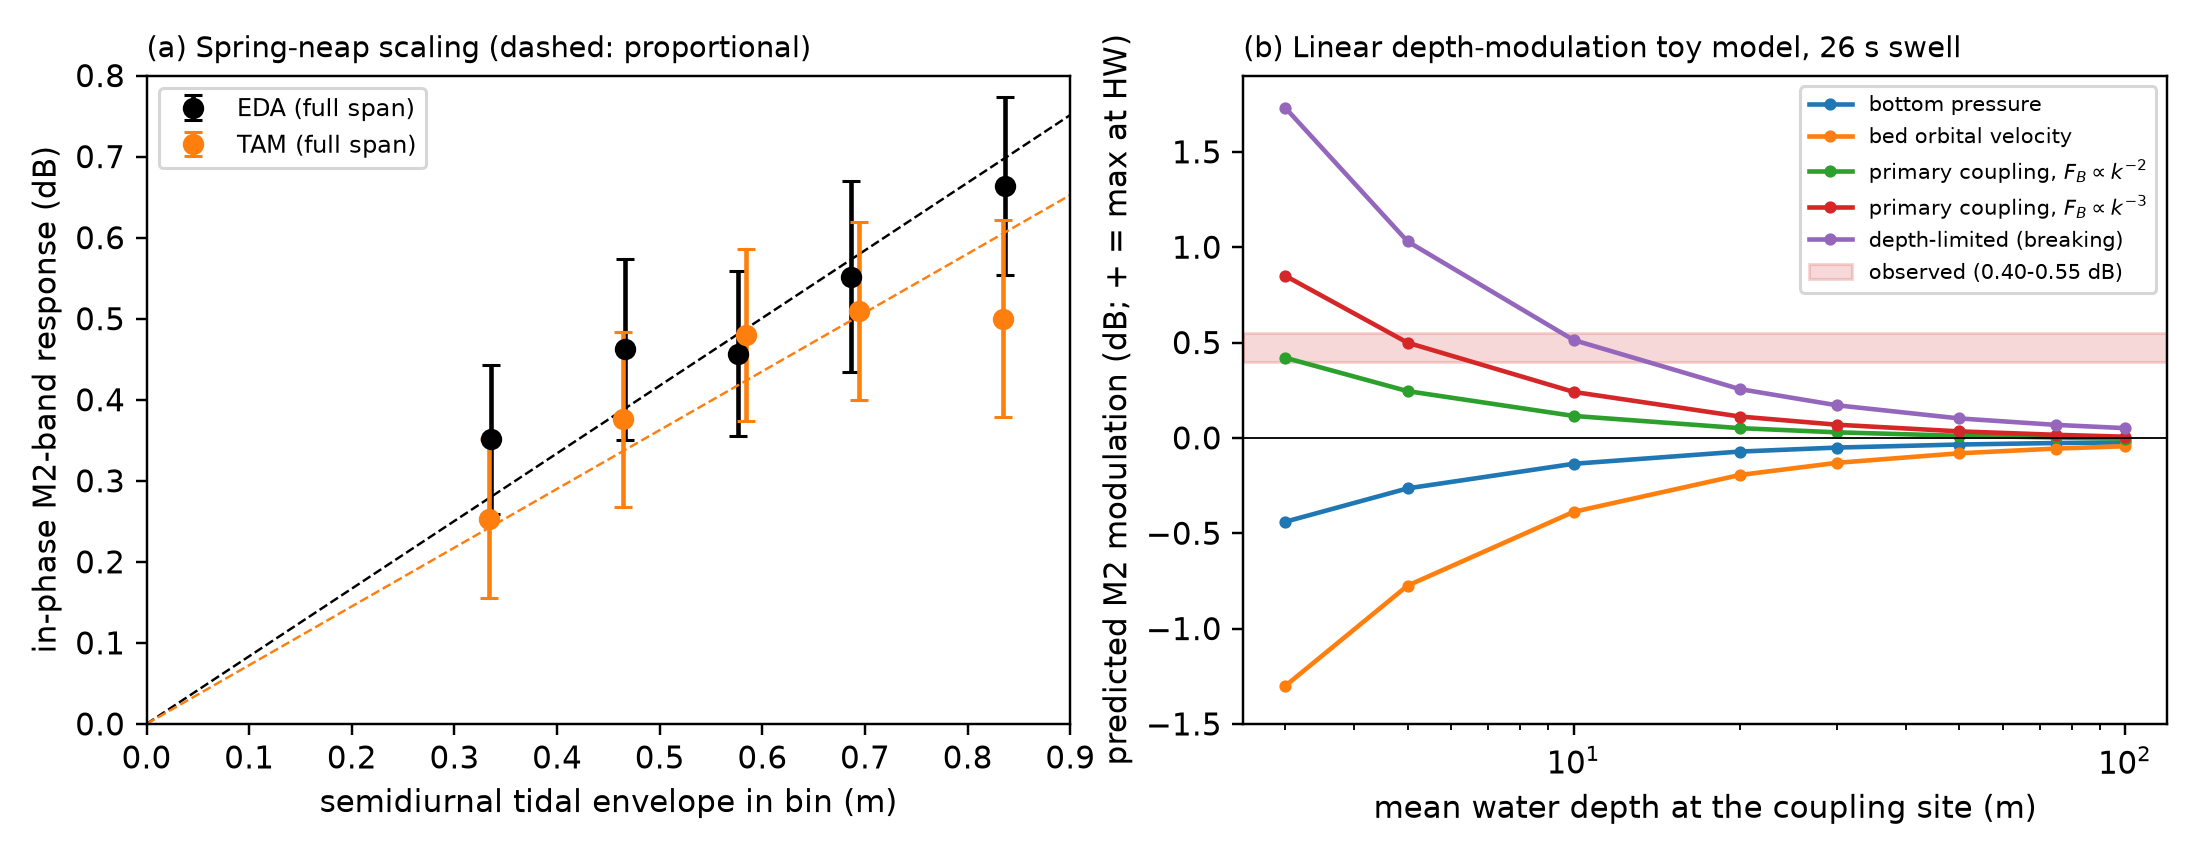
\includegraphics[width=\textwidth]{figs/fig4_springneap_model.png}
\caption{(a) In-phase M2 response of LMB power in five bins of semidiurnal tidal range (envelope) at EDA (2019--2026) and TAM (2022--2026), with $\pm1.96$ standard errors and proportional fits (dashed). (b) Toy-model M2 modulation for 26 s swell under a 0.59 m M2 tide, as a function of mean water depth at the coupling site (positive: maximum at high water). The shaded band is the observed 0.40--0.55 dB range.}
\label{fig:sn}
\end{figure}

\end{document}
